%--------------------
% Packages
% -------------------
\documentclass[12pt,a4paper]{article}
% \usepackage[a4paper, left=15mm, right=15mm, top=15mm, bottom=15mm]{geometry}
\usepackage[utf8x]{inputenc}
\usepackage[T1]{fontenc}
%\usepackage{gentium}
\usepackage{mathptmx} % Use Times Font
% \usepackage[siunitx]{circuitikz} % for circuit schematics
\usepackage{siunitx}
\usepackage{amsmath} % for the equation* environment
\usepackage{graphicx}
\usepackage{pgfplots}
\pgfplotsset{compat=1.14}
\usepackage{float}

\usepackage{graphicx} % Required for including pictures % clashes with circuitikz
% \usepackage[swedish]{babel} % Swedish translations
\usepackage[pdftex,linkcolor=black,pdfborder={0 0 0}]{hyperref} % Format links for pdf
\usepackage{calc} % To reset the counter in the document after title page
\usepackage{enumitem} % Includes lists

\frenchspacing % No double spacing between sentences
\linespread{1.2} % Set linespace
\usepackage[a4paper, lmargin=0.08\paperwidth, rmargin=0.08\paperwidth, tmargin=0.08\paperheight, bmargin=0.08\paperheight]{geometry} %margins
%\usepackage{parskip}
% \usepackage[all]{nowidow} % Tries to remove widows
\usepackage[protrusion=true,expansion=true]{microtype} % Improves typography, load after fontpackage is selected

\usepackage[inkscapelatex=false]{svg}
\graphicspath{ {./media/} }

% \pagecolor{black}
% \color{white}

\usepackage{setspace}


%-----------------------
% Set pdf information and add title, fill in the fields
%-----------------------
\hypersetup{ 	
pdfsubject = {},
pdftitle = {ee5311-2025-ee24s053-pwc-report-tut5},
pdfauthor = {Karthik B K <ee24s053@smail.iitm.ac.in>}
}

%-----------------------
% Begin document
%-----------------------
\begin{document}

\title{EE5311 \\ Report of Practical Work Conducted for Tutorial 06 (b)}
\author{Karthik B K ee24s053}
\maketitle

\section{Experiment A}
\subsection{Layout Insporation}
In the course EE5333, we wrote a sequence pair floorplanner. I plugged the standard cell dimensions into that floorplanner to get some inspiration for the layout structure.
\begin{center}
    \begin{tabular}{ccc}
     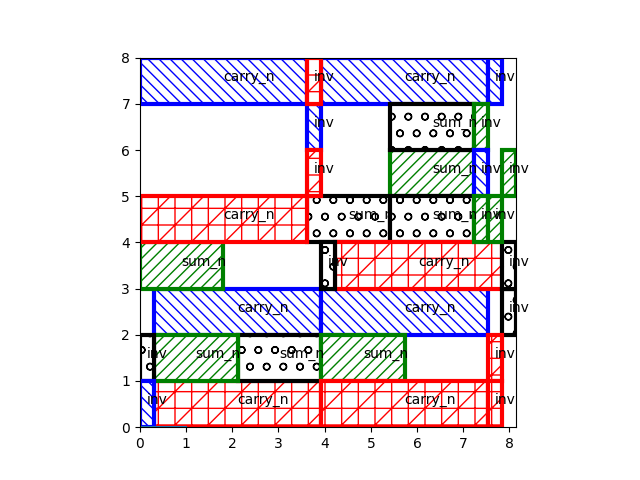
\includegraphics[width=0.32\linewidth]{tut6/reports/media/fp_inspo_1.png} &
     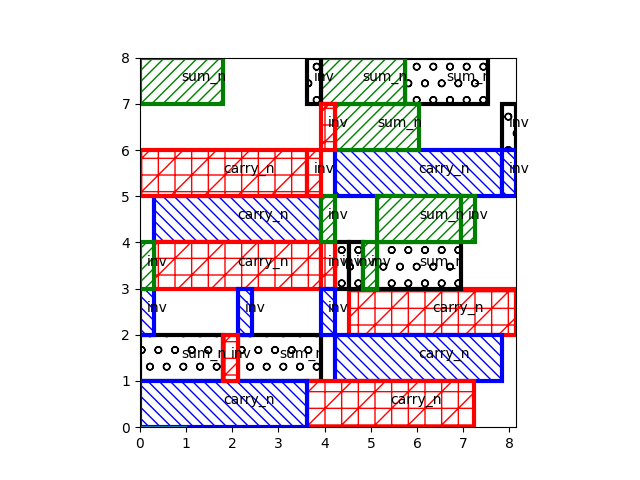
\includegraphics[width=0.32\linewidth]{tut6/reports/media/fp_inspo_2.png} &
     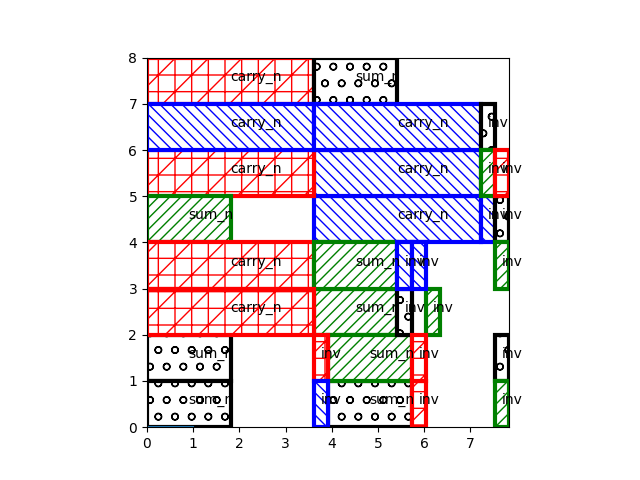
\includegraphics[width=0.32\linewidth]{tut6/reports/media/fp_inspo_3.png} \\
     Fig 0a: Inspiration 1 & Fig 0b: Inspiration 2 & Fig 0c: Inspiration 3
\end{tabular}
\end{center}
\subsection{Layouts}
\noindent We draw inspiration from the above floorplans and create the following layout using \emph{klayout}.
\begin{center}
     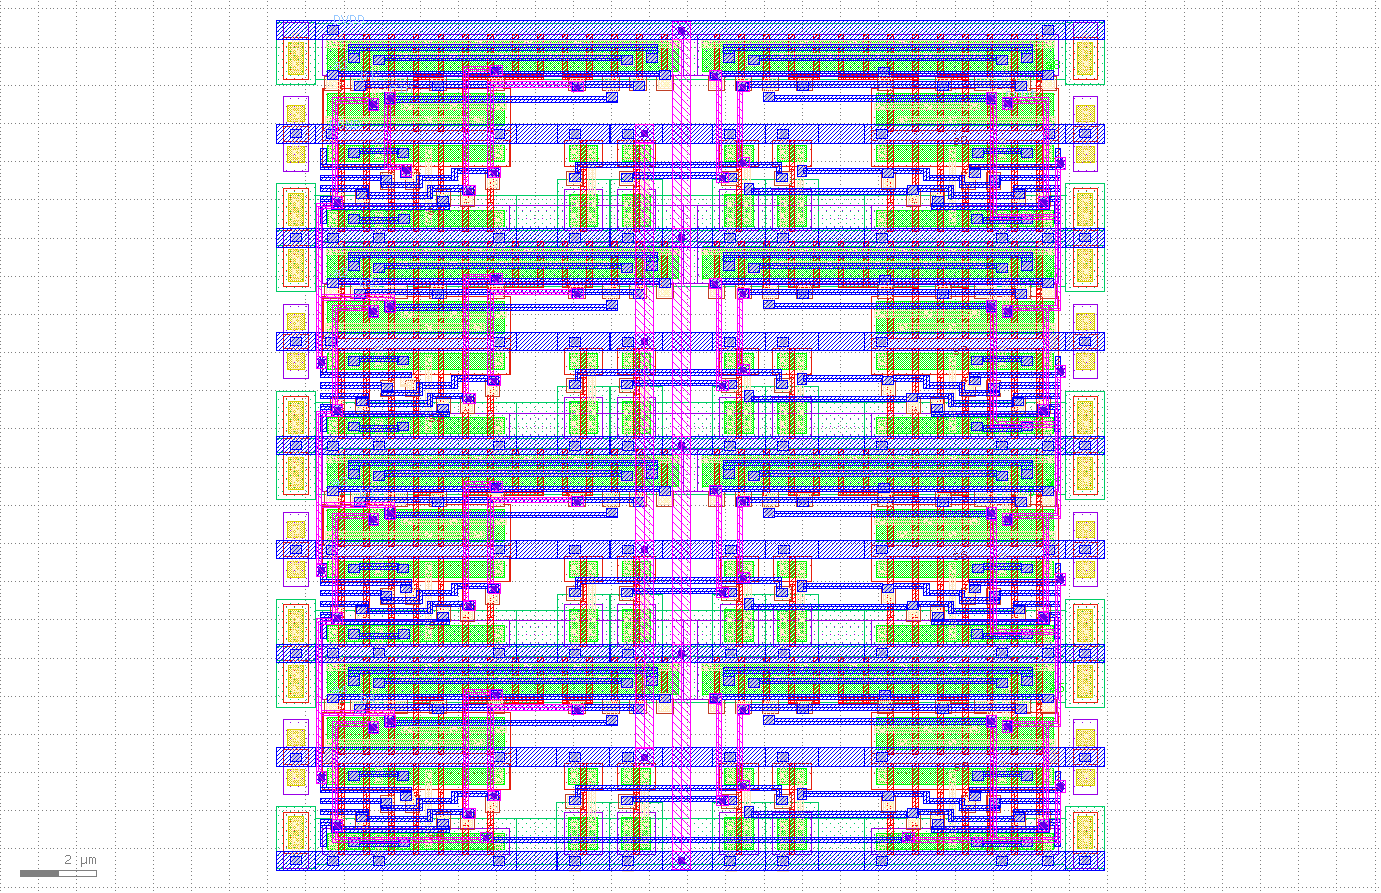
\includegraphics[width=0.99\linewidth]{tut6/rca/rca8b.gds.png} \\
     Fig 1a: Layout of the 8-bit Ripple Carry Adder
\begin{tabular}{cc}
     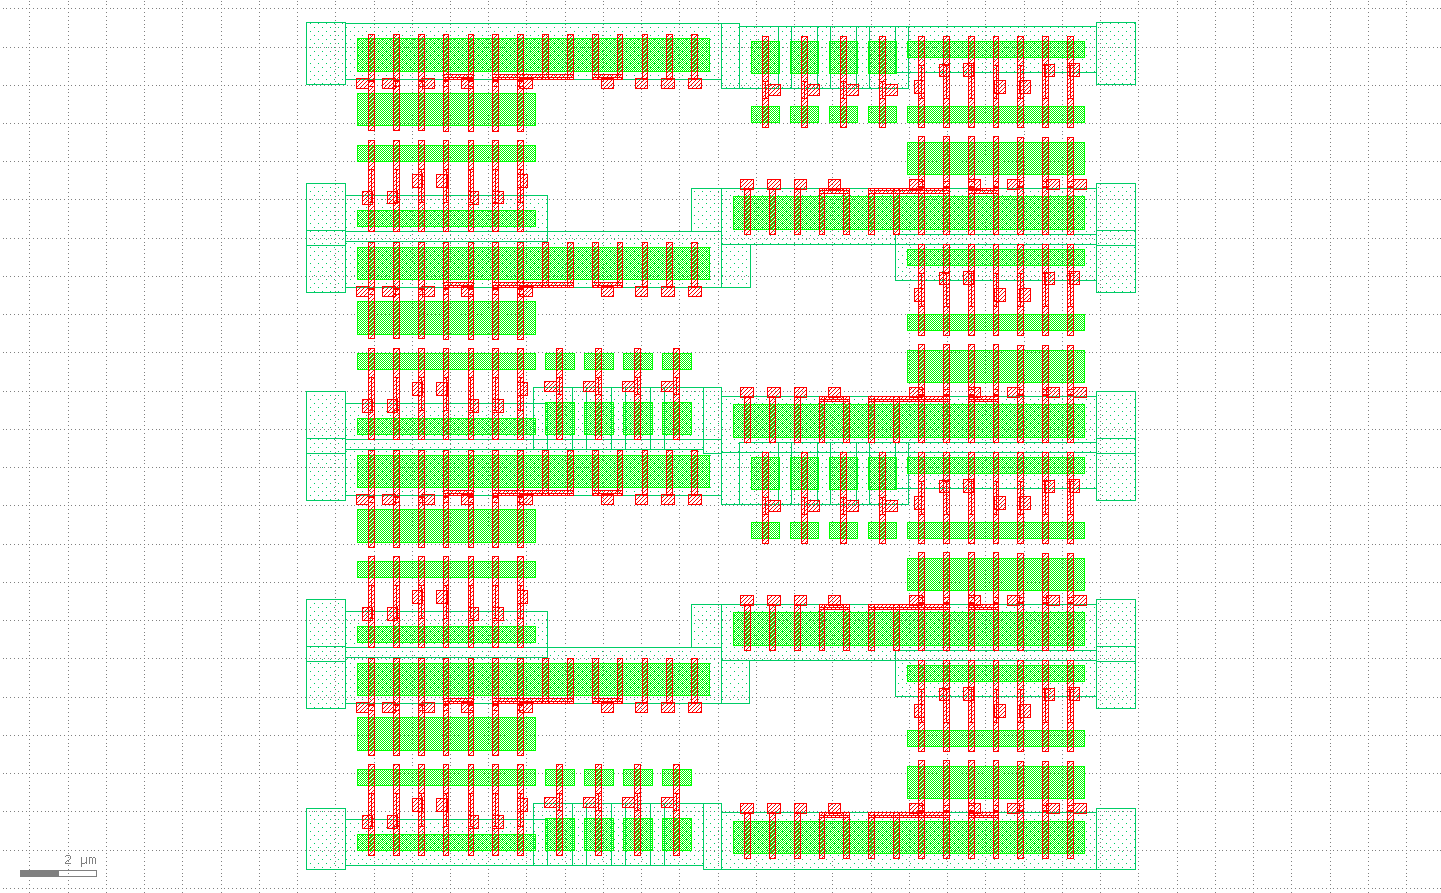
\includegraphics[width=0.48\linewidth]{tut6/rca/rca8b.mos.gds.png} &
     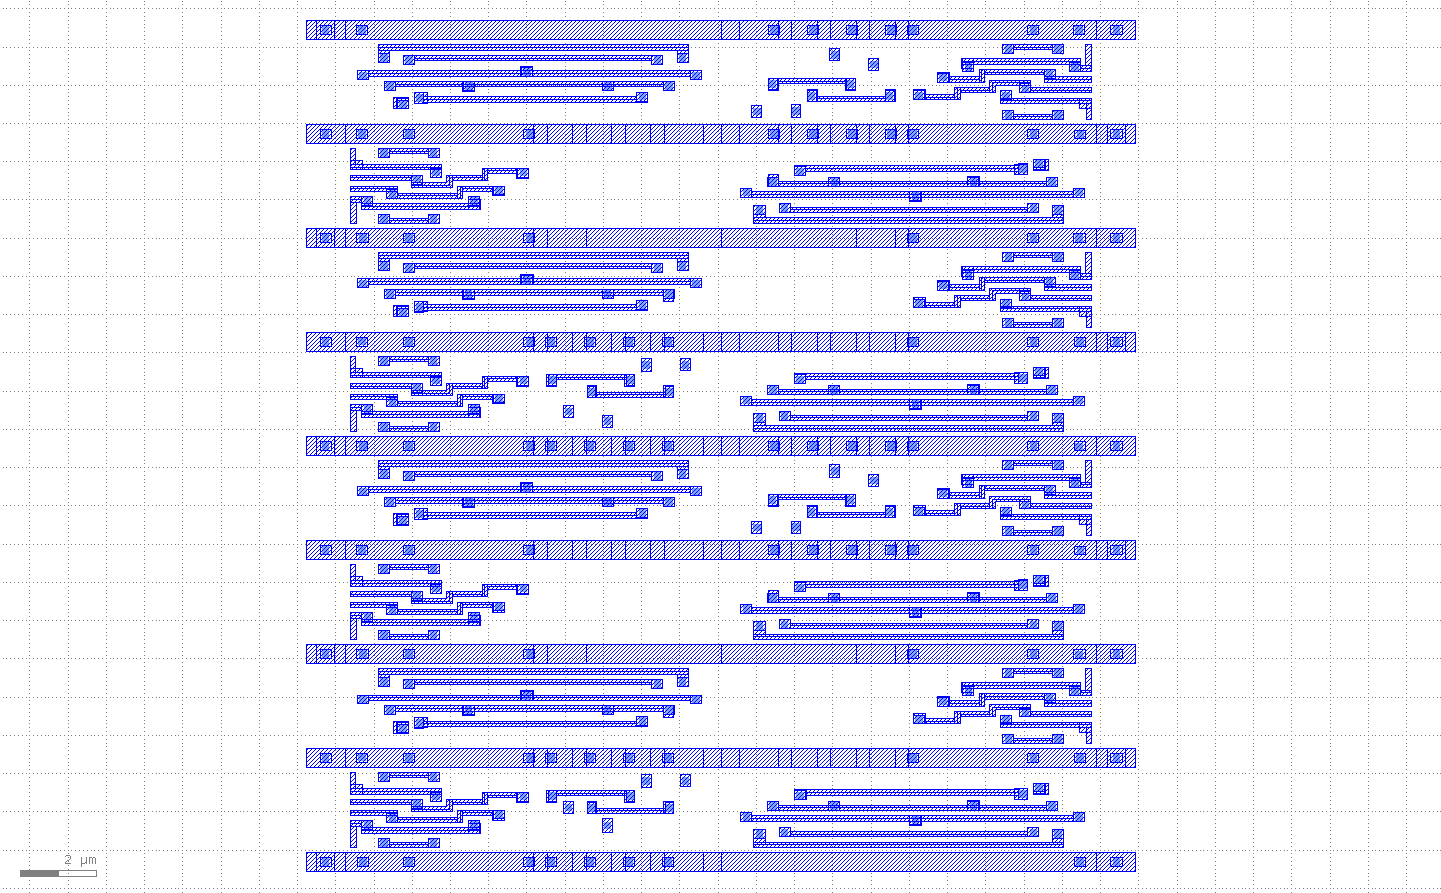
\includegraphics[width=0.48\linewidth]{tut6/rca/rca8b.m1.gds.png} \\
     Fig 1b: N-Well, Diff and Poly layers shown & Fig 1c: M1 layer shown
\end{tabular}
    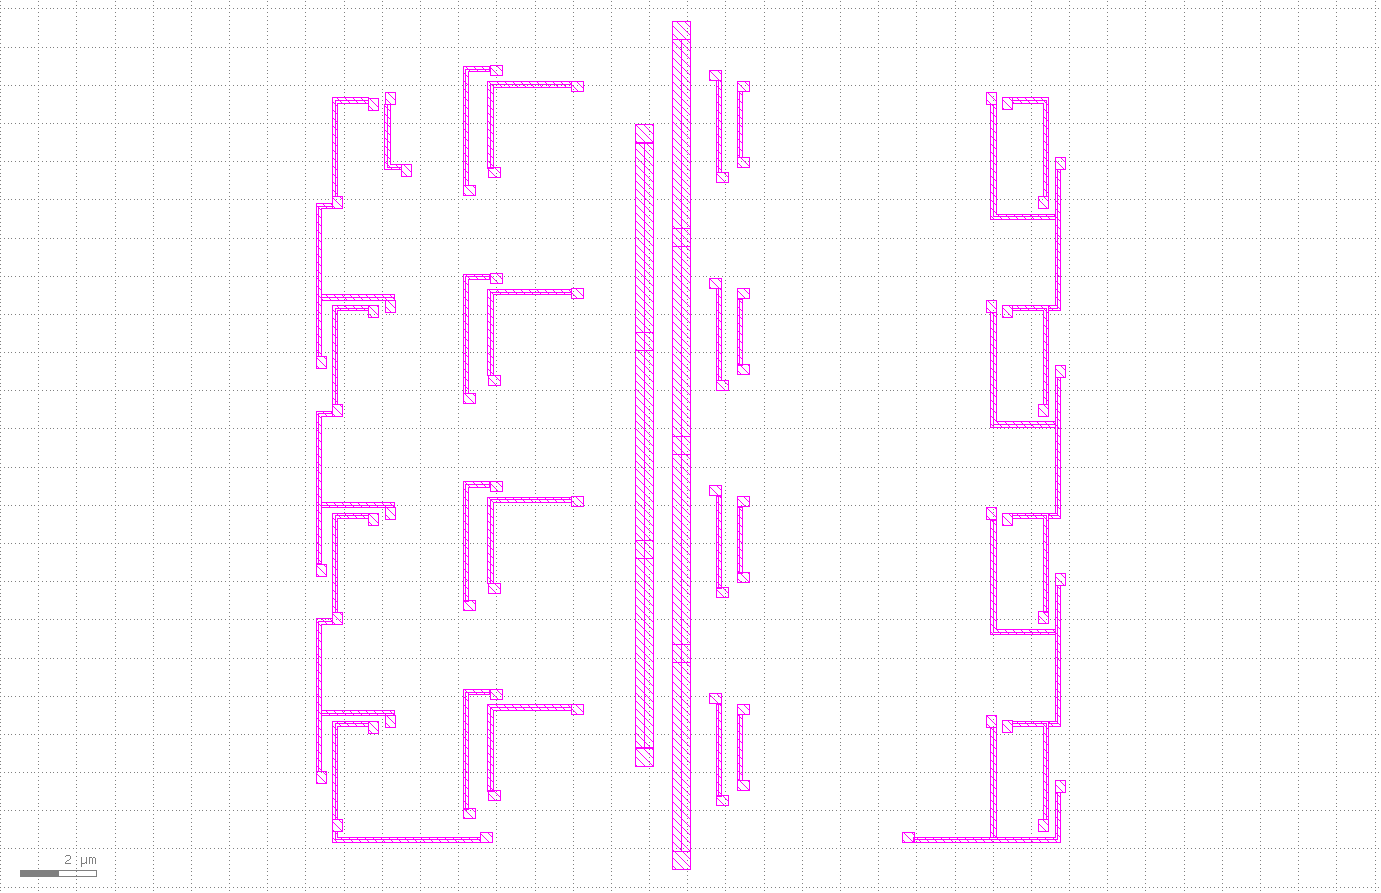
\includegraphics[width=0.48\linewidth]{tut6/rca/rca8b.m2.gds.png} \\ Fig 1d: M2 layer shown
\end{center}

\noindent All routing outside the adder cells themselves were strictly restricted to the Metal 2 layer only.The layout is DRC and LVS clean. Total width (including tap cells on both sides) is 21.7 um, and total height inclusive of the power grid is 22.24 um. Width excluding tap cells on both sides is 19.66 um. \\
\noindent Aspect ratio (W/H) if tap cells are excluded, is 0.88, and if tap cells are included, is 1.10.

\subsection{Measurements}
\noindent We perform a transient simulation with the setup both before and after layout extraction for the inverter and obtain the following plots.
\begin{center}
\begin{tabular}{cc}
     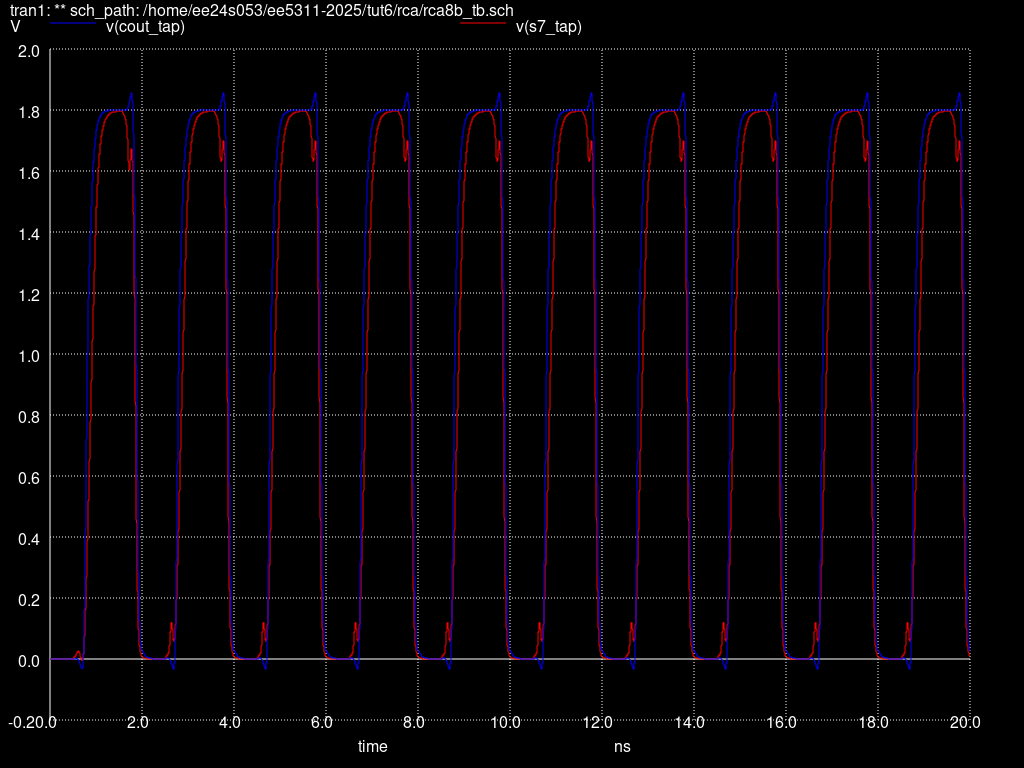
\includegraphics[width=0.47\linewidth]{tut6/rca/pre-layout-waveforms.png} &
     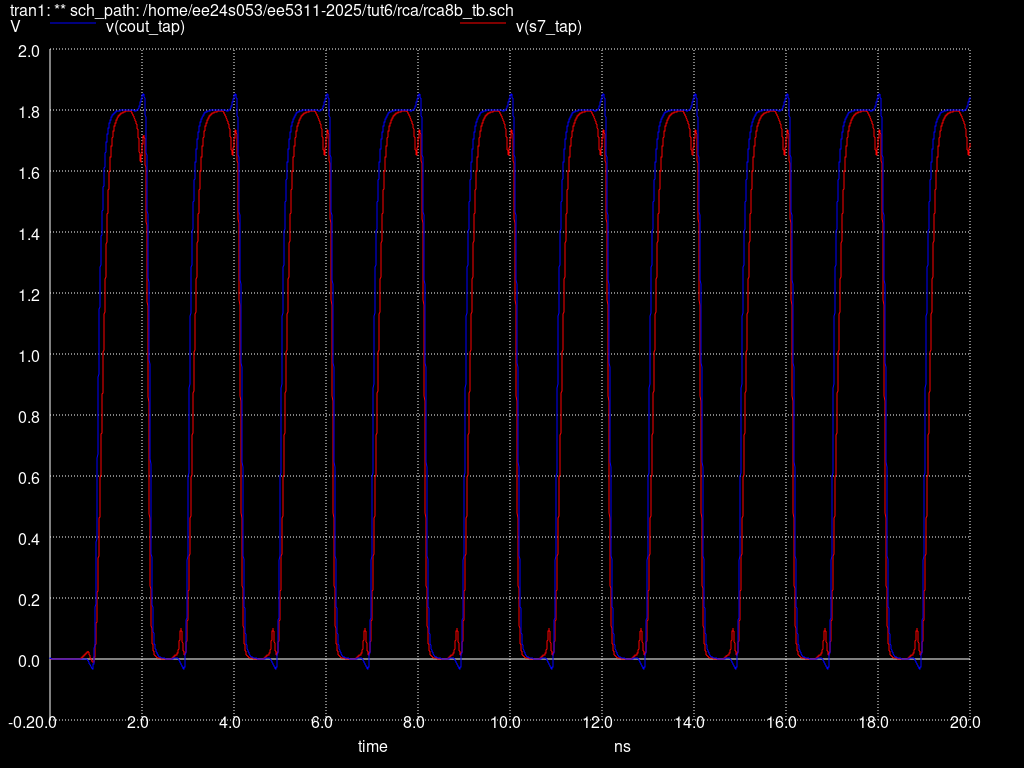
\includegraphics[width=0.47\linewidth]{tut6/rca/post-layout-waveforms.png} \\
     Fig 5a: Output signals from the 8-bit Adder pre-layout & Fig 5b: Output signals from the adder post-layout
\end{tabular}
\end{center}
\noindent We obtain the following values for period and frequency without the layout parasitics.
\begin{verbatim}
tlh_carry           =  8.035678e-10 targ=  8.060678e-10 trig=  2.500000e-12
thl_carry           =  8.763952e-10 targ=  1.883895e-09 trig=  1.007500e-09
carry delay: 8.39981E-10
tlh_sum             =  8.976240e-10 targ=  9.001240e-10 trig=  2.500000e-12
thl_sum             =  8.479798e-10 targ=  1.855480e-09 trig=  1.007500e-09
sum delay: 8.72802E-10
\end{verbatim}
\noindent We obtain the following values for period and frequency when we include the layout parasitics.
\begin{verbatim}
tlh_carry           =  1.048991e-09 targ=  1.051491e-09 trig=  2.500000e-12
thl_carry           =  1.160816e-09 targ=  2.168316e-09 trig=  1.007500e-09
carry delay: 1.10491E-09
tlh_sum             =  1.143346e-09 targ=  1.145846e-09 trig=  2.500000e-12
thl_sum             =  1.130393e-09 targ=  2.137893e-09 trig=  1.007500e-09
sum delay: 1.13687E-09
\end{verbatim}

\section{Declarations}
\begin{enumerate}
    \item I have publicly hosted this work on GitHub to help reproduce all of my results. The same can be accessed through the following \href{https://github.com/iamkarthikbk/ee5311-2025}{\underline{link}}.
\end{enumerate}

\end{document}
